%% 
%% Copyright 2007-2020 Elsevier Ltd
%% 
%% This file is part of the 'Elsarticle Bundle'.
%% ---------------------------------------------
%% 
%% It may be distributed under the conditions of the LaTeX Project Public
%% License, either version 1.2 of this license or (at your option) any
%% later version.  The latest version of this license is in
%%    http://www.latex-project.org/lppl.txt
%% and version 1.2 or later is part of all distributions of LaTeX
%% version 1999/12/01 or later.
%% 
%% The list of all files belonging to the 'Elsarticle Bundle' is
%% given in the file `manifest.txt'.
%% 
%% Template article for Elsevier's document class `elsarticle'
%% with harvard style bibliographic references

\documentclass[preprint,12pt,authoryear]{elsarticle}

%% Use the option review to obtain double line spacing
%% \documentclass[authoryear,preprint,review,12pt]{elsarticle}

%% Use the options 1p,twocolumn; 3p; 3p,twocolumn; 5p; or 5p,twocolumn
%% for a journal layout:
%% \documentclass[final,1p,times,authoryear]{elsarticle}
% \documentclass[final,1p,times,twocolumn,authoryear]{elsarticle}
%% \documentclass[final,3p,times,authoryear]{elsarticle}
% \documentclass[final,3p,times,twocolumn,authoryear]{elsarticle}
%% \documentclass[final,5p,times,authoryear]{elsarticle}
%% \documentclass[final,5p,times,twocolumn,authoryear]{elsarticle}

\usepackage{amsmath}
\usepackage{amsfonts}
\usepackage{amssymb}
\usepackage{url,hyperref,lineno,microtype,subcaption}
\usepackage{color,tensor,multirow,siunitx}
\usepackage[onehalfspacing]{setspace}
\usepackage{makecell}
\renewcommand{\cellalign}{cl}
\usepackage{caption}
\captionsetup[figure]{name=Fig., labelfont=bf}

\renewcommand{\cellalign}{cl}

\newcommand{\ds}{\displaystyle}
\newcommand{\nl}{\ \\ }
\newcommand{\ud}{\textrm{ d}}
\newcommand{\bs}{\bigskip}

\newcommand{\bu}{\mathbf{u}}
\newcommand{\bv}{\mathbf{v}}
\newcommand{\bx}{\mathbf{x}}
\newcommand{\be}{\mathbf{e}}
\newcommand{\bb}{\mathbf{b}}
\newcommand{\bk}{\mathbf{k}}
\newcommand{\bn}{\mathbf{n}}
\newcommand{\bR}{\mathbf{R}}

\definecolor{red}{rgb}{1,0,0}
\definecolor{blue}{rgb}{0,0,0.8}
\definecolor{green}{rgb}{0,0.5,0}
\newcommand{\emphc}[1]{\emph{\textcolor{red}{#1}}}
\newcommand{\modif}[1]{\textcolor{red}{#1}}
\newcommand{\hycom}{\textsc{hycom} }
\newcommand{\ie}{{\it i.e.}\ }
\newcommand{\eg}{{\it e.g.}\ }
\newcommand{\edit}[1]{\textcolor{orange}{#1}}
\newcommand{\UV}{\mathbf{U}}


\journal{Ocean Modelling}

\begin{document}

\begin{frontmatter}

%% Title, authors and addresses

%% use the tnoteref command within \title for footnotes;
%% use the tnotetext command for theassociated footnote;
%% use the fnref command within \author or \affiliation for footnotes;
%% use the fntext command for theassociated footnote;
%% use the corref command within \author for corresponding author footnotes;
%% use the cortext command for theassociated footnote;
%% use the ead command for the email address,
%% and the form \ead[url] for the home page:
%% \title{Title\tnoteref{label1}}
%% \tnotetext[label1]{}
%% \author{Name\corref{cor1}\fnref{label2}}
%% \ead{email address}
%% \ead[url]{home page}
%% \fntext[label2]{}
%% \cortext[cor1]{}
%% \affiliation{organization={},
%%            addressline={}, 
%%            city={},
%%            postcode={}, 
%%            state={},
%%            country={}}
%% \fntext[label3]{}

\title{Impacts of Hurricane Irma (2017) on ocean transport processes}

%% use optional labels to link authors explicitly to addresses:
%% \author[label1,label2]{}
%% \affiliation[label1]{organization={},
%%             addressline={},
%%             city={},
%%             postcode={},
%%             state={},
%%             country={}}
%%
%% \affiliation[label2]{organization={},
%%             addressline={},
%%             city={},
%%             postcode={},
%%             state={},
%%             country={}}

\author[eli]{Thomas Dobbelaere\corref{corr}}
\ead{thomas.dobbelaere@uclouvain.be}
\author[rsmas]{Milan Curcic}
\author[cimas,aoml]{Matthieu le H\'enaff}
\author[eli,immc]{Emmanuel Hanert}
\cortext[corr]{Corresponding author}

\affiliation[eli]{
    organization={Eath and Life Institute (ELI), UCLouvain},
    % addressline={}, 
    city={Louvain-la-Neuve},
    % postcode={1348}, 
    % state={},
    country={Belgium}
}
\affiliation[rsmas]{
    organization={Rosenstiel School of Marine and Atmospheric Sciences (RSMAS), University of Miami},
    % addressline={}, 
    city={Coral Gables},
    % postcode={1348}, 
    state={Florida},
    country={USA}
}
\affiliation[cimas]{
    organization={Cooperative Institute for Marine and Atmospheric
    Studies (CIMAS), University of Miami},
    % addressline={}, 
    city={Miami},
    % postcode={1348}, 
    state={Florida},
    country={USA}
}
\affiliation[aoml]{
    organization={Atlantic Oceanographic and Meteorological Laboratory
    (AOML), NOAA},
    % addressline={}, 
    city={Miami},
    % postcode={1348}, 
    state={Florida},
    country={USA}
}
\affiliation[immc]{
    organization={Institute of Mechanics, Materials and Civil Engineering (IMMC), UCLouvain},
    % addressline={}, 
    city={Louvain-la-Neuve},
    % postcode={1348}, 
    % state={},
    country={Belgium}
}

\begin{abstract}
    Tropical cyclones are becoming more intense and more frequent. Their effect is particularly acute in coastal areas where they cause extensive damage leading to an influx of debris, sediments and waste to the sea. However, most coastal ocean models do not represent their transport correctly as they do not couple the hydrodynamics with the wind-generated waves. This may lead to significant errors in heavy-wind conditions. Here, we investigate current-wave interactions during a major cyclone and assess their impact on transport processes. We do that by coupling the unstructured-mesh coastal ocean model SLIM with the spectral wave model SWAN, and applying it to the Florida Reef Tract during Hurricane Irma (Sept. 17). We show that the coupled model successfuly reproduces the wave behaviour, the storm surge and the ocean currents during the passage of the hurricane. We then use the coupled and uncoupled wave-current model to simulate the transport of passive drifters. We show that the wave force alone can lead to changes of up to 1 m/s in the modelled currents, which in turn lead to differences of up to 10 km in the position of drifting material over the duration of the hurricane. \textcolor{red}{[Add a sentence on Stokes drift vs wave-current coupling]}. Our results suggest that wave-current interactions can strongly impact the transport of drifting material such as sediments and debris in the aftermath of a hurricane. They should thus be taken into account in order to correctly assess its overall impact
\end{abstract}

%%Graphical abstract
% \begin{graphicalabstract}
% %\includegraphics{grabs}
% \end{graphicalabstract}

%%Research highlights
% \begin{highlights}
% \item Research highlight 1
% \item Research highlight 2
% \end{highlights}

\begin{keyword}
%% keywords here, in the form: keyword \sep keyword

%% PACS codes here, in the form: \PACS code \sep code

%% MSC codes here, in the form: \MSC code \sep code
%% or \MSC[2008] code \sep code (2000 is the default)

\end{keyword}

\end{frontmatter}

\linenumbers

\section{Introduction}

% Wave-current interactions in coastal areas are of great importance for coastal engineering and management as they play a key role in sediment transport, morphological evolution and pollutant mixing \citep{bever2013simulating, li1998three}. However, these interactions are highly nonlinear and can vary significantly in space and time \citep{wu2011fvcom}. Wave-induced currents are generated by wave radiation stress gradients \citep{longuet1970longshore}, affecting water levels near shorelines and wave breaking points \citep{longuet1964radiation}. Changes in water levels and currents, in turn, affect the motion and evolution of the waves \citep{sikiric2013coupling}. Coupled wave-current models are therefore required to correctly represent these complex interactions.

% As coastal oceans are characterized by a complex topography with islands, inlets and estuaries, unstructured models are preferred as structured grid models show limitations in resolving topologically-controlled nearshore processes \citep{wu2011fvcom, chen2007finite}. Being able to capture the impact of topology on wave interactions becomes even more important in the case of hurricanes. The strong hurricane-induced winds generate large wind-waves and disturb ocean conditions \citep{liu2020impacts} by causing coastal upwellings on continental shelves \citep{smith1982response} and inducing strong currents, waves and storm surges in nearshore and coastal regions \citep{dietrich2010high, weisberg2006hurricane}. 

% South Florida and the Gulf of Mexico are particularly vulnerable to hurricanes \citep{malmstadt2009florida} and modelling studies predict tropical cyclones to increase both in frequency and intensity in this region \citep{marsooli2019climate, knutson2010tropical}. Accurately representing wave-current interactions under strong winds becomes therefore critical in order to predict hurricane impacts in events such such as the Deepwater Horizon oil spill in the Gulf of Mexico in 2010 \citep{le2012surface}. A better description of the impacts of waves on currents could also improve the accuracy of search and rescue efforts during storms \citep{breivik2013advances} or inform reef managers by better understanding the impact of hurricane-induced currents on larval dispersal \citep{lugo2001inferring}.

% Individual-based modelling of particulates has been extensively used to study the transport of drifting materials such as pollutants, sediments or larvae \citep{le2012surface,liubartseva2018tracking, figueiredo2013synthesizing,frys2020fine}. Although some of these studies take the impact of waves into account by adding a Stokes drift velocity, \ie the net drift of a floating particle in the direction of the wave propagation \citep{van2018stokes}, to the Eulerian currents, they usually neglect the wave-induced currents. Such practice is reasonable in the case of fair weather, when wave-induced forces exerted on currents are relatively small, but might lead to significant inaccuracies during storm conditions \citep{rohrs2012observation,curcic2016hurricane}. To assess the importance of wave-current interactions during a tropical cyclone, we investigated the transport of drifting particles on the Florida shelf during Hurricane Irma, one of the strongest and costliest tropical cyclones on record in the Atlantic Basin \citep{xian2018brief}, which made landfall in Florida in September 2017.

% In this study, we developed an unstructured coupled wave-current model of South Florida to simulate the ocean circulation during hurricane Irma. Both modelled currents and waves were validated against field measurements and were then used to simulate the transport of drifting material in the Florida Keys and the Florida inner shelf during the passage of the hurricane. Model outputs were then compared with uncoupled simulation results in order to assess the impact of wave-induced forces and Stokes drift on the modelled currents and transports.

Tropical cyclones are becoming more intense and more frequent \citep{bhatia2019recent, kossin2020global}. This increase is likely due to climate change and will probably continue in the future \citep{knutson2020tropical}. However, estimating the impact of tropical cyclones on the coastal ocean circulation remains a challenge. Understanding wave-current interactions and being able to represent their impact on coastal ocean transport processes is central to many coastal activities such as dredging, erosion management, O\&G, search and rescue \citep{bever2013simulating,li1998three, breivik2013advances}. \textcolor{red}{[Add 1/2 sentences]}

Wave-current interactions during a cyclone are highly nonlinear and can vary significantly in space and time \citep{wu2011fvcom}. Wave-induced currents are generated by wave radiation stress gradients \citep{longuet1970longshore}, affecting water levels near shorelines and wave breaking points \citep{longuet1964radiation}. Changes in water levels and currents, in turn, affect the motion and evolution of the waves \citep{sikiric2013coupling}. Coupled wave-current models are therefore required to capture these complex interactions. \textcolor{red}{[Add 1/2 sentences]}

Coastal oceans are characterized by the complex topography of the coastline and the presence of islands, reefs and artificial structures. Traditional structured-grid models often lack the flexibility to simulate near-shore processes at a sufficiently small scale. Instead, unstructured-mesh models can easily adapt to the topography and are hence better suited to coastal processes \citep{wu2011fvcom, chen2007finite}. Being able to capture the impact of the topography on wave interactions becomes even more important in the case of tropical cyclones. Heavy winds generate large wind-waves and disturb ocean conditions \citep{liu2020impacts} by causing coastal upwellings on continental shelves \citep{smith1982response} and inducing strong currents, waves and storm surges in nearshore and coastal regions \citep{dietrich2010high, weisberg2006hurricane}. 

The transport of drifting objects or substances that are locally released is often best represented by a Lagrangian individual-based model. Such an approach is routinely used to model the dispersal of larvae, pollutants, sediments and many other tracers (e.g. \cite{le2012surface,liubartseva2018tracking, figueiredo2013synthesizing,frys2020fine}). Although some transport models take the impact of waves into account by adding a Stokes drift velocity, \ie the net drift of a floating particle in the direction of the wave propagation \citep{van2018stokes}, to the Eulerian currents, they usually neglect the wave-induced currents. Such practice is reasonable in the case of fair weather, when wave-induced forces exerted on currents are relatively small, but might lead to significant errors during storm conditions \citep{rohrs2012observation,curcic2016hurricane}. 

The objective of this study is therefore to assess the importance of wave-current interactions during a tropical cyclone. We investigate the transport of drifting particles on the Florida shelf during Hurricane Irma, one of the strongest and costliest tropical cyclones on record in the Atlantic Basin \citep{xian2018brief}, which made landfall in Florida in September 2017. To do that, we developed an unstructured coupled wave-current model of South Florida to simulate the ocean circulation during hurricane Irma. Both modelled currents and waves were validated against field measurements and were then used to simulate the transport of drifting material in the Florida Keys and the Florida inner shelf. Model outputs were then compared with uncoupled simulation results in order to assess the impact of wave-induced forces and Stokes drift on the modelled currents and transports.  

% === METHODS === %
\section{Methods}
\subsection{Study area and observational data}
The large-scale ocean circulation around South Florida is dominated by the Florida Current (FC), which originates from the Loop Current (LC) where it enters the Florida Straits from the Gulf of Mexico, and, downstream, forms the Gulf Stream. The FC is a major western boundary current characterized by spatial variability and meandering, associated with the presence of cyclonic eddies between the core of the current and the complex reef topography of the Florida Reef Tract (FRT) \citep{lee1995florida,kourafalou2012florida}.
% The northern half of these reefs are made of early Holocene reef frameworks and indurated sand ridges while the southern part (the Florida Keys) is composed of a chain of limestone islands, fossilized remnants of ancient coral reefs and sand bars \citep{hoffmeister1968geology,shinn1988geology,lidz1991paleoshorelines}.
The variability of the FC extends over a large range of spatial and temporal scales, with periods of 30-70 days in the Lower Keys \citep{lee1995florida} and shorter periods of 2-21 days in the Upper Keys \citep{lee1977low}, and exhibits significant seasonal and interannual cycles \citep{johns1987meandering, lee1988wind,schott1988variability}. Circulation on the West Florida Shelf (WFS) on the other hand is forced by local winds and tidal fluctuations \citep{lee2002volume,liu2012seasonal}. \textcolor{red}{[Add sentences on tropical cyclones in that area]}

The state of the ocean around Florida is monitored by an extensive array of tide gauges, current meters and buoys. In this study, we used sea surface elevation measurements from the National Oceanic and Atmospheric Administration’s (NOAA) Tides and Currents dataset. These measurements were taken at four locations: two in the Florida Keys (Key West and Vaca Key); one on the eastern coast of Florida (Virginia Key); and one on the western coast (Naples). For the currents, we used ADCP measurements from the University of South Florida's College of Marine Science's (USF/CMS) Coastal Ocean Monitoring and Prediction System (COMPS) for the WFS \citep{weisberg2009mean}. More specifically, we used measurements from moorings C10, C12 and C13, respectively located at the 25, 50, and 50 m isobaths of the WFS \citep{liu2020impacts}. Finally, for the waves, we used measurements from four buoys of the NOAA's National Data Buoy Center (NDBC); two on Florida's eastern shelf and two on the WFS. The locations of all measurement stations are shown in Fig. \ref{fig:mesh}A,C.

\begin{figure}
    \centering
    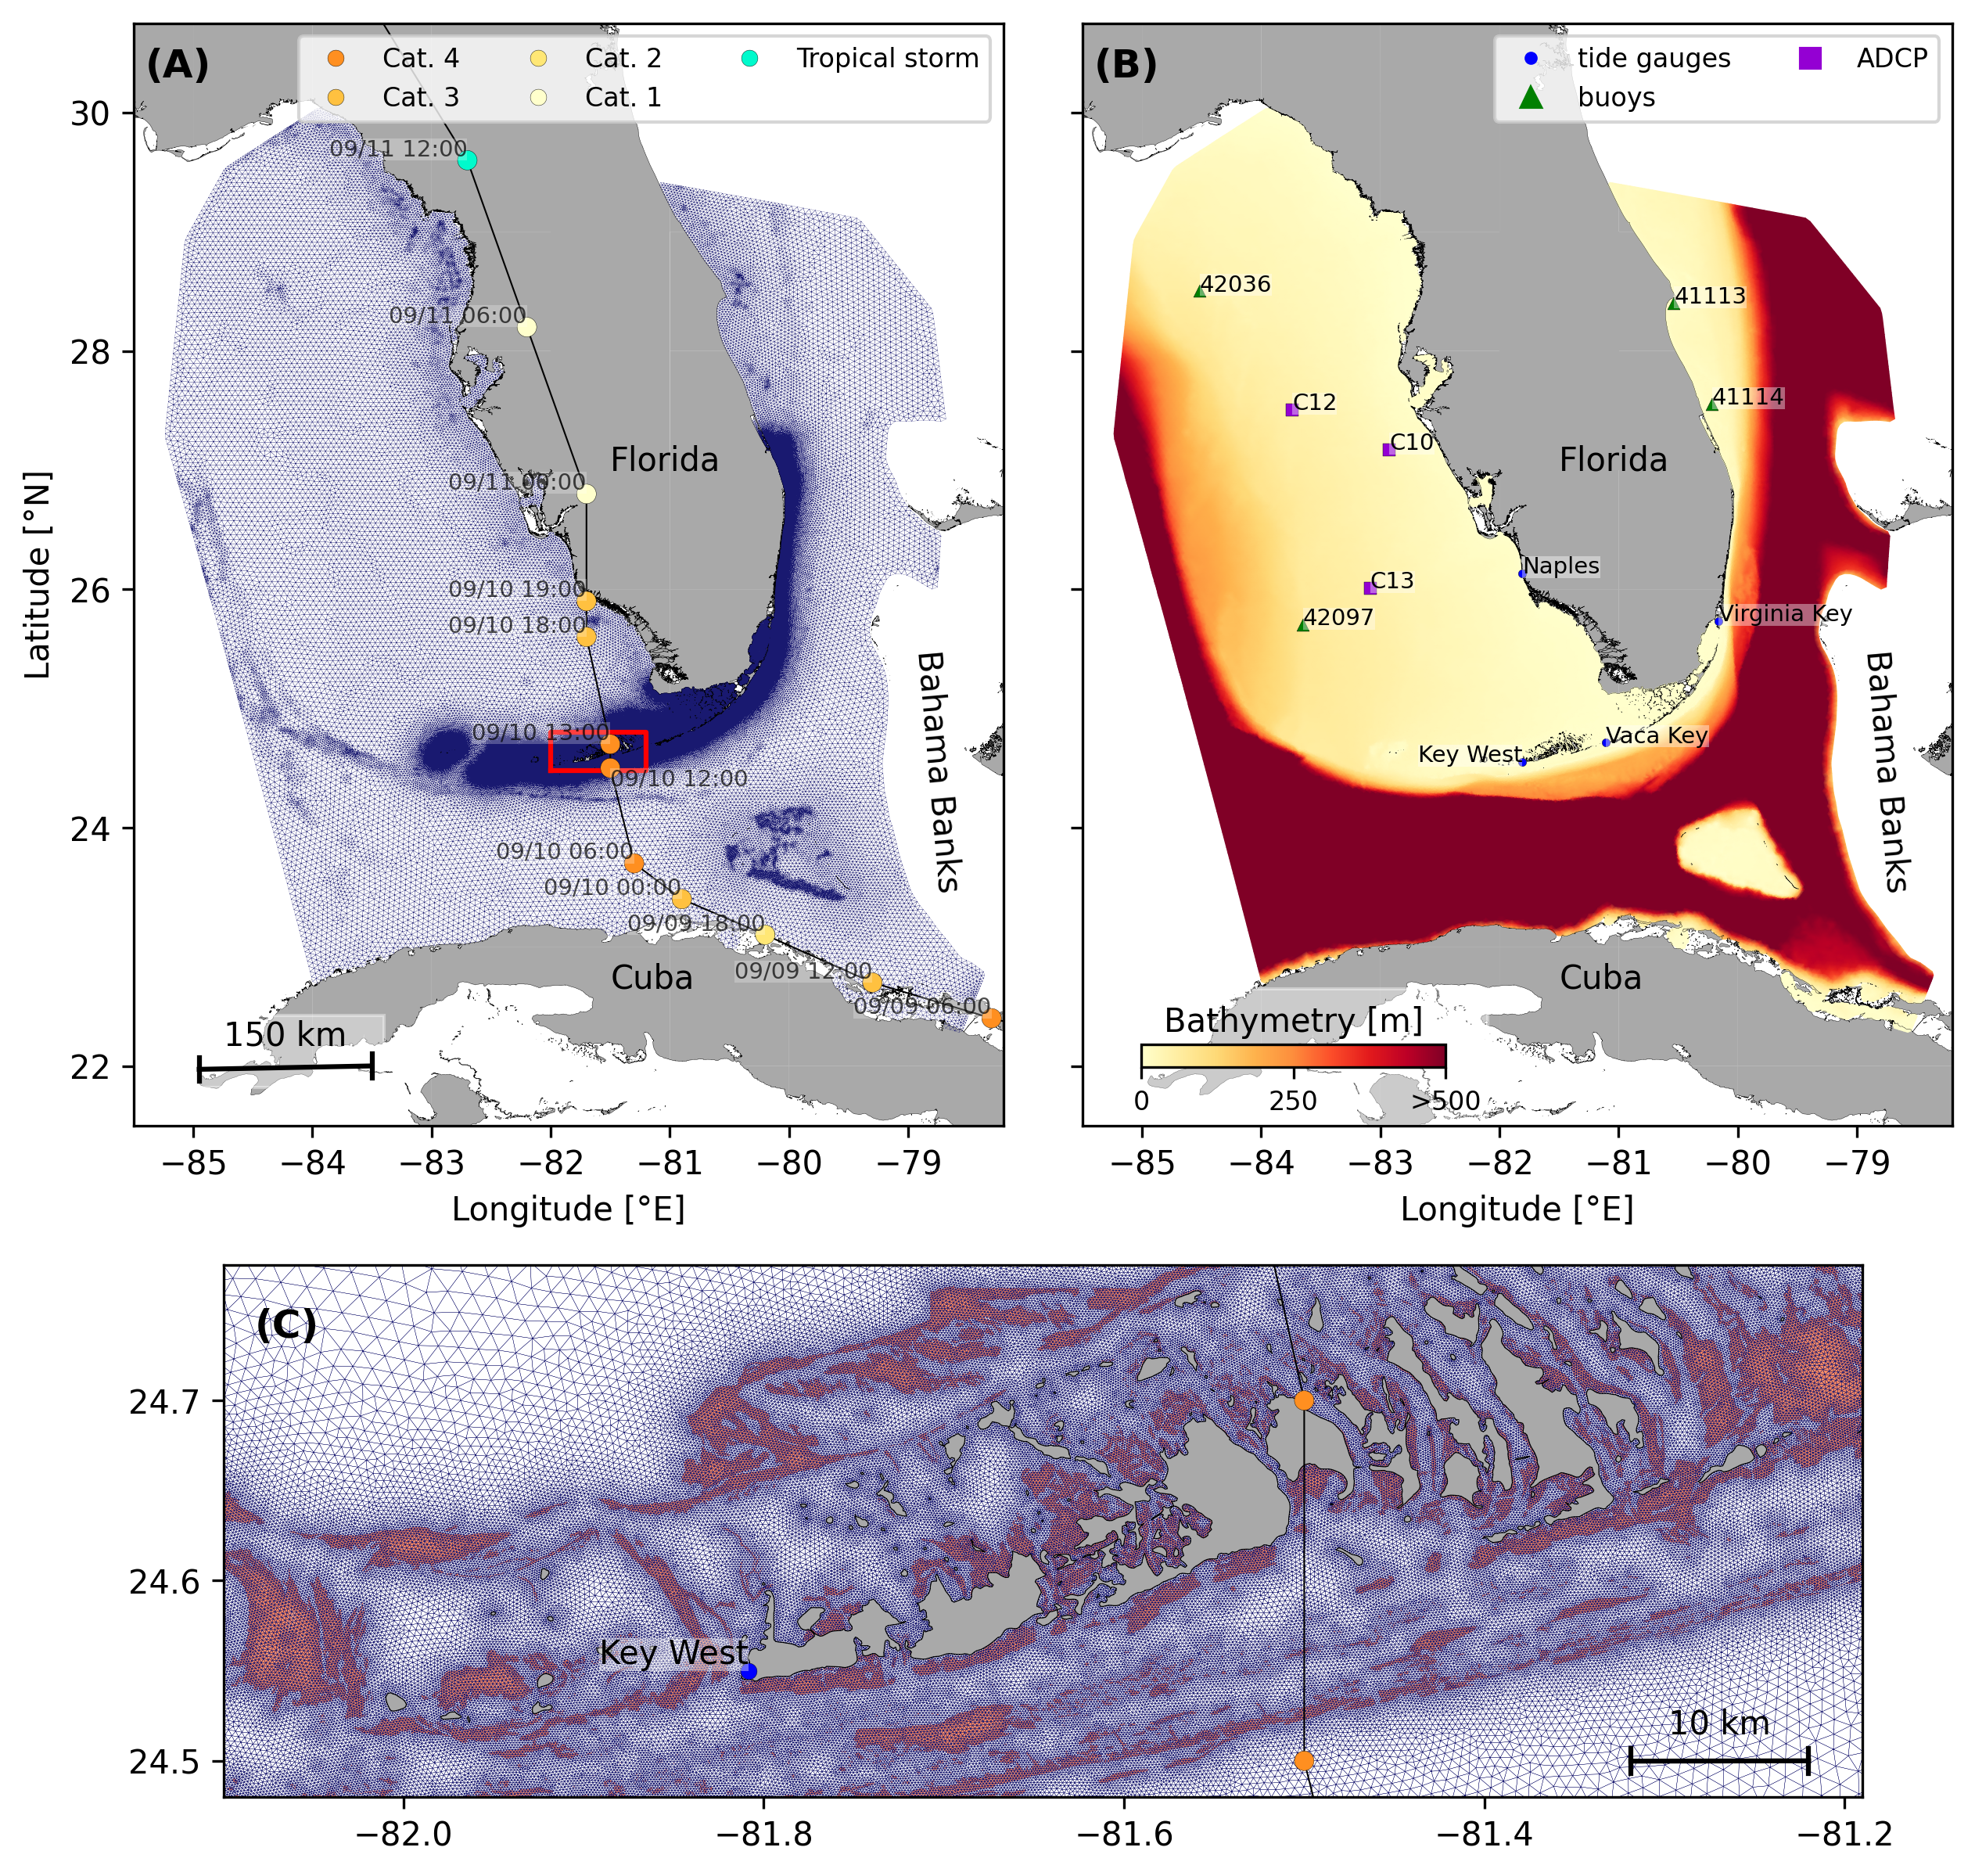
\includegraphics[width=\textwidth]{fig/fig_mesh_hurr.png}
    \caption{(\textbf{A}) Mesh of the computational domain with the trajectory of Irma, category of the hurricane is given by the Saffir-Simpson color scale. (\textbf{B}) Bathymetry of the domain with the location of stations used for the validation of the model outputs. (\textbf{C}) Close up view of the Lower Keys area, where the mesh resolution reaches 100m near reefs (shown in dark orange) and islands (highlighted in dark grey)}
    \label{fig:mesh}
\end{figure}

\subsection{Wind and atmospheric pressure during Hurricane Irma}

Irma made landfall in Florida on 10 September 2017 as a category 3 hurricane, first at Cudjoe Key (Florida Keys) and later on Marco Island, south to Naples (see hurricane track in Fig. \ref{fig:mesh}). It then weakened to a category 2 hurricane as it moved further inland \citep{pinelli2018overview}. The storm damaged up to 75\% of the buildings at its landfall point in the Florida Keys, making it one of the strongest and costliest hurricanes on record in the Atlantic basin \citep{xian2018brief,zhang2019modeling}. The strongest reported wind speed was 50 m/s on Marco Island while the highest recorded storm surge was 2.3 m, although larger wind speed likely occurred in the Florida Keys \citep{pinelli2018overview}. In order to reproduce the wind profile of Irma in our model, we used high-resolution H$^\ast$Wind wind fields \citep{powell1998hrd}. As these data represent 1-min averaged wind speeds, we multiplied them by a factor 0.93 to obtain 10-min averaged wind speeds \citep{harper2010guidelines}, which are more consistent with the time step of our model. Furthermore, H*Wind wind profiles did not cover the whole model extent during the passage of the hurricane and were thus blended within coarser wind field extracted from ECMWF ERA-5 datasets (Fig. \ref{fig:atm}A). The pressure field during the passage of Hurricane Irma was also reconstructed using ERA-5 data. However, the coarse resolution of the dataset smoothes out the depression at the center of the hurricane, leading to an underestimation of the pressure gradient (Fig. \ref{fig:atm}B). To better capture the central depression of Irma, we therefore built a hybrid pressure field using the position and the minimal pressure of the core of the hurricane based on its track as recorded in the HURDAT 2 database \citep{landsea2013atlantic}. Based on this information, the hybrid pressure field was constructed by combining an idealized Holland pressure profile \citep{lin2012hurricane} within the radius of maximum wind speed of Irma \citep{knaff2018statistical} with ERA-5 pressure field. The transition from the Holland profile to ERA-5 data outside the radius of maximum wind speed data was performed using a smooth step function (Fig. \ref{fig:atm}).

\begin{figure}
    \centering
    \includegraphics[width=.99\textwidth]{fig/hwind_vs_era.png}
    \includegraphics[width=.99\textwidth]{fig/holland_vs_era.png}
    \caption{Snapshot of the hybrid wind (\textbf{A}) and pressure (\textbf{B}) profiles constructed to capture the passage of Hurricane Irma at 1800 UTC on 9 September 2017. Wind profiles are obtained by combining high resolution H*Wind with coarser ERA-5 wind fields. The pressure field is built by combining the ERA-5 pressure field with an idealized Holland pressure profile based on the track of Irma in the HURDAT 2 database. Holland field was only used within the radius of maximum wind speed (dashed grey line) of the hurricane to capture its central depression. }
    \label{fig:atm}
\end{figure}

\subsection{Hydrodynamic model}

Ocean currents generated during hurricane Irma around South Florida were modelled using the 2D barotropic version of the unstructured-mesh coastal ocean model SLIM\footnote{\url{https://www.slim-ocean.be}}. The model mesh covers an area similar to the model extent of \cite{dobbelaere2020coupled}, that includes the FRT but also the Florida Straits and part of the Gulf of Mexico (Figure \ref{fig:mesh}). However, this area has been slightly extended northeastward and westward in order to include the NOAA-NDBC buoys. Furthermore, to withstand potential cell drying during the hurricane, we solved the conservative shallow water equations with wetting-drying:
\begin{equation}
    \begin{split}
        \dfrac{\partial H}{\partial t} +\nabla\cdot(\UV) =& ~0~, \\
        \dfrac{\partial \UV}{\partial t}  + \nabla\cdot\left(\dfrac{\UV\UV}{H}\right) =& -f\mathbf{e}_z \times \UV + \alpha gH\nabla(H-h) - \dfrac{1}{\rho}\nabla p_\text{atm} + \dfrac{1}{\rho}\text{\boldmath$\tau$}_s \\
         &+\nabla\cdot(\nu\nabla\UV) - \dfrac{C_b}{H^2}|\UV|\UV + \gamma(\UV_\text{ref}-\UV)~,
    \end{split} \label{eq:slim}
\end{equation}
where $H$ is the water column height and $\UV$ is the depth-averaged transport; $f$ is the Coriolis coefficient; $g$ is the gravitational acceleration; $h$ is the bathymetry; $\alpha$ is a coefficient stating whether the mesh element is wet ($\alpha=1$) or dry ($\alpha=0$) \citep{le2020implicit}; $\nu$  is the viscosity; $C_b$ is the bulk bottom drag coefficient; $p_\text{atm}$ is the atmospheric pressure; {\boldmath$\tau$}$_s$ is the surface stress, usually due to wind; and $\gamma$ is a relaxation coefficient towards a reference transport $\UV_\text{ref}$. As in \cite{frys2020fine} and \cite{dobbelaere2020coupled}, SLIM currents were gradually relaxed towards the operational Navy \hycom product (GOMl0.04\footnote{\url{https://www.hycom.org/data/goml0pt04}}, \cite{chassignet2007hycom}) in regions where the water depth exceeds 50m.

At very high wind speeds, the white cap is blown off the crest of the waves. This phenomenon, also known as spumes, has been hypothesized to generate a layer of droplets that acts as a slip layer for the winds at the ocean-atmosphere interface \citep{holthuijsen2012wind}. It causes a saturation of the wind drag coefficient for strong winds \citep{powell2003reduced,donelan2004limiting,curcic2020revised}. We take this saturation effect into account by using the wind  drag parameterization of \cite{moon2007physics}. In this parameterization, the drag coefficient $C_d$ depends on the wind speed at 10-m height $U_{10}$ according to:
\begin{equation}
    C_d = \kappa^2 \log\left(\dfrac{10}{z_0}\right)^{-2}\label{eq:drag}
\end{equation}
where $\kappa$ is the von Karman constant and $z_0$ is the roughness length expressed as: 
\begin{equation}
    z_0 =\left\{\begin{array}[]{ll}
        \dfrac{0.0185}{g}U_{\ast}^2 & \text{if }U_{10} \leq 12.5\text{ m/s}~, \\
        \lbrack 0.085(-0.56U_{\ast}^2+20.255U_{\ast} & \text{if }U_{10} > 12.5\text{ m/s}~, \\
        \quad +2.458) - 0.58\rbrack\times 10^{-3} 
    \end{array}\right.
\end{equation}
with $U_\ast$ the friction velocity. The relation between $U_{10}$ and $U_{\ast}$ is given by:
\begin{equation}
    U_{10}=-0.56U_{\ast}^2+20.255U_{\ast}+2.458~.
\end{equation}

The mesh resolution depends on the distance to the coastlines and reefs following the approach of \cite{dobbelaere2020coupled}. The mesh is then further refined according to bathymetry value and gradient, as suggested in the SWAN user-guide\footnote{\url{http://swanmodel.sourceforge.net/unswan/unswan.htm}}. Such an approach improves the model efficiency as the mesh resolution is only increased where required by the currents and waves dynamics. The mesh was generated with the seamsh\footnote{\url{https://pypi.org/project/seamsh/}} Python library, which is based on the the open-source mesh generator GMSH \citep{geuzaine2009gmsh}. It is composed of approximately 7.7 $\times$ 10$^5$ elements. The coarsest elements, far away from the FRT, has a characteristic length of about 5 km whereas the finest elements have a characteristic length of about 100 m along the coastlines and over the reefs (Fig \ref{fig:mesh}).

\subsection{Wave model}
Waves were modelled using the parallel unstructured-mesh version of the Simulating WAves Nearshore (SWAN) model \citep{booij1999third}, one of the most popular wave models for coastal areas and inland waters. It solves the action balance equation \citep{mei1989applied}:
\begin{equation}
    \dfrac{\partial N}{\partial t} + \nabla_\mathbf{x}\cdot[(\mathbf{c}_g+\mathbf{u})N] + \dfrac{\partial }{\partial \theta}[c_\theta N] + \dfrac{\partial}{\partial \sigma}[c_\sigma N] = \dfrac{S_{in}+S_{ds}+S_{nl}}{\sigma}~, \label{eq:swan}
\end{equation}
where $N=E/\sigma$ is the wave action density and $E$ is the wave energy spectrum; $\theta$ is the wave propagation direction; $\sigma$ is the intrinsic wave frequency; $\mathbf{c}_g$ is the wave group velocity, $\mathbf{u}=\mathbf{U}/H$ is SLIM depth-averaged current velocity; $c_\theta$ and $c_\sigma$ are the propagation velocities in spectral space due to refraction and shifting in frequency due to variations in depth and currents; and $S_{in}$, $S_{ds}$, and $S_{nl}$ respectively represent wave growth by wind, wave decay and nonlinear transfers of wave energy through interactions between triplets and quadruplets. The wave spectra were discretized with 48 direction bins and 50 frequency bins logarithmically distributed from 0.03 to 2 Hz. Exponential wind growth was parameterized using the formulation of \cite{janssen1991quasi}, while dissipations by whitecapping and bottom dissipations followed the formulations of \cite{komen1984existence} and \cite{madsen1989spectral}, respectively. Coefficients for exponential wind growth and whitecapping parameterizations were based on the results of \cite{siadatmousavi2011evaluation}, and significantly differ from SWAN's default settings. By default, SWAN implements the wind input formulation of \cite{komen1984existence} and the steepness-dependent coefficient governing dissipation by whitecapping is a linear function of the wave number. In this study, this steepness-dependent coefficient is a quadratic function of the wave number, as it showed better predictions of the significant wave height in the study of \cite{siadatmousavi2011evaluation}. The choice of these formulations was motivated by the appearance of numerical instabilities in the region of the Gulf Stream when using SWAN's default parameter values. Finally, wave boundary conditions were derived from WAVEWATCH III \citep{tolman2009user} spectral outputs at NDBC buoy locations. We selected these datasets as the large number of NDBC buoys around our region of interest allowed for a fine representation of the wave spectra on the boundary of the domain. 

Surface waves induce a net drift in the direction of the wave propagation, known as the Stokes drift \citep{van2018stokes,stokes1880theory}. This net drift has a significant impact on sediment transport in nearshore regions \citep{hoefel2003wave}, on the formation of Langmuir cells \citep{langmuir1938surface, craik1976rational} as well as on the transport of heat, salt or pollutants such as oil or micro-plastic in the upper ocean layer \citep{mcwilliams2000vertical,rohrs2012observation,drivdal2014wave}. To correctly model the Stokes drift profile in mixed wind-driven sea and swell conditions, the full two-dimensional wave spectrum must be represented by a spectral wave model within a wave-current coupling \citep{van2018stokes}. We therefore used SWAN modelled spectra to compute the Stokes drift as follows:
\begin{equation}
    \mathbf{u}_{s} = \int_0^{2\pi}\int_0^{+\infty} \dfrac{\sigma^3}{h\tanh(2kh)}E(\sigma,\theta)(\cos\theta, \sin\theta)d\sigma d\theta~, \label{eq:stokes}
\end{equation}
where $k$ is the norm of the wave vector; $h$ is the water depth; and $E(\sigma,\theta)$ is the wave energy density.

\subsection{Coupled model}

SLIM and SWAN are coupled so that they run on the same computational core and the same unstructured mesh. SLIM is run first and passes the wind velocity ($\mathbf{U}_{10}$), water level ($\eta=H-h$) and depth-averaged current ($\mathbf{u}=\mathbf{U}/H$) fields to SWAN, as well as a roughness length ($z_0$) for the bottom dissipation formulation of \cite{madsen1989spectral}. This roughness length is computed from SLIM's bulk drag coefficient $C_b$ following the approach of \cite{dietrich2011hurricane} so that both models have consistent bottom dissipation parameterizations. SWAN then uses these quantities to compute the wave radiation stress gradient, that is then passed to SLIM as the force exerted by waves on currents {\boldmath$\tau$}$_\text{wave}$ (Fig. \ref{fig:coupling}). SLIM then uses this quantity to update the value of the surface stress {\boldmath$\tau$}$_s$ in Eq. (\ref{eq:slim}), that now becomes the sum of wind and wave-induced stresses $\text{\boldmath$\tau$}_s = \text{\boldmath$\tau$}_\text{wind}+\text{\boldmath$\tau$}_\text{wave}$. Here, the momentum flux from the atmosphere to the ocean is taken as the commonly-used full wind tress {\boldmath$\tau$}$_\text{wind}$. Doing so, we neglect the momentum advected away from the storm by the waves, leading to a 10-15\% overestimation of the momentum flux in hurricane winds \citep{curcic2015explicit}. Moreover, we followed the approach of \cite{dietrich2012performance} by characterizing the wave-induced stresses using the radiation-stress representation instead of the vortex-force representation \citep{mcwilliams2004asymptotic}. Although the later provides a clearer and more meaningful decomposition of the wave effect, we implemented the first representation for the sake of simplicity as it allows us to provide the whole wave contribution as an additional surface stress to SLIM \citep{lane2007wave}.

SLIM's governing equations are integrated using an implicit time integration scheme while SWAN is unconditionally stable \citep{dietrich2012performance}, allowing both models to be run with relatively large time steps. In this study, the stationary version of SWAN was used, \ie the time derivative of Eq. \ref{eq:swan} was set to zero. This resulted in reduced scaling and convergence rates than with the nonstationary version of SWAN but increased the stability of the model. The wave spectra at each node of the mesh was saved at the end of each iteration to serve as initial conditions for the next one. Both models were run sequentially using a time step of 600 s, so that each computational core was alternatively running either SLIM or SWAN. As in the coupling between SWAN and ADCIRC \citep{dietrich2012performance}, both models use the same local sub-mesh, allowing for a one-to-one correspondence between the geographic locations of the mesh vertices. No interpolation is therefore needed when passing the discretised variables from one model to the other, which allows an efficient inter-model communication. However, as SLIM is based on  a discontinuous Galerkin finite element method, an additional conversion step to a continuous framework was required to transfer SLIM nodal quantities to SWAN.  

\begin{figure}
    \centering
    \includegraphics[width=.99\textwidth]{fig/coupling_v2.png}
    \caption{Schematic illustration of the coupled SLIM+SWAN model.}
    \label{fig:coupling}
\end{figure}

\subsection{Quantifying the effect of wave-current interactions on transport}\label{sec:traj}

To quantify the impact of wave-current interactions on transport processes, we compared the trajectories of passive particles advected by the uncoupled SLIM and coupled SLIM+SWAN currents during the passage of Irma in the Lower Keys. Furthermore, the depth-averaged Stokes drift was computed using the wave spectra of the coupled model SLIM+SWAN run as well as those of an uncoupled SWAN run. Particles were released on the inner and outer shelves at the points highlighted By red and blue dots in Fig. \ref{fig:init} on Sept. 7 at 0000 UTC and then tracked until Sept. 15. These initial particle positions were found using backtracking methods \citep{dobbelaerereport} to ensure that the release particles would intersect the path of Irma during its passage through the Florida Keys. We first defined two 25 km$^\text{2}$ circular regions on the trajectory of the hurricane (see red and blue circles in Fig. \ref{fig:init}). Particles within these two regions were then tracked backward in time using uncoupled SLIM currents from the exact time of the passage of the hurricane until Sept. 7 at 0000 UTC. Their positions at the end of the backward simulation (see red and blue particle clouds in Fig. \ref{fig:init}) corresponds to the initial condition of the forward transport simulations described below. We then compared the trajectories of particles originating from these regions and advected forward in time by different sets of currents: (i) uncoupled SLIM currents alone; (ii) coupled SLIM+SWAN currents; (iii) SLIM currents with the addition of the depth-averaged Stokes drift computed with the coupled wave-current model (Stokes-C); (iv) SLIM+SWAN currents with Stokes-C; and (v) SLIM currents with the depth-averaged Stokes drift computed with the uncoupled wave model (Stokes-U). Particles trajectories are compared by computing the distances between the centers of mass of the particle clouds through time.

\begin{figure}
    \centering
    \includegraphics[width=.9\textwidth]{fig/inner_outer_regions.png}
    \caption{Release regions of the passive particles on the inner and outer shelves (red and blue clouds) obtained by backtracking particles released in the red and blue circular areas during the passage of Irma.}
    \label{fig:init}
\end{figure}

%%%%%%%%%%%%%%%%%%%
% --- RESULTS --- %
%%%%%%%%%%%%%%%%%%%
\section{Results}

We first validated the reconstructed atmospheric fields of hurricane Irma as well as the outputs of our coupled wave-current model against field measurements. A summary of the error statistics is given in Table \ref{tab:stat}. We then used the validated model outputs to simulate the transport of passive drifters in the Lower Keys during the passage of Hurricane Irma. These drifters were advected by the sets of currents described in section \ref{sec:traj} and their trajectories were compared to evaluate the impact of the wave-current interactions and the Stokes drift on the transport processes during the passage of Irma.

\subsection{Model validation}

H*Wind winds and hybrid pressure field agree well with station measurements at Vaca Key station (Fig. \ref{fig:forcings}). The hybrid pressure field shows a better agreement with observations than ERA-5 pressure as it successfully reproduces the storm depression. ERA-5 fields, on the other hand, fail to reproduce the low pressure at the core of the hurricane due to their coarser grid, leading to an overestimation of 8 mbar of the storm depression. Both H*Wind and ERA-5 agree well with observed wind speeds although both data sets tend to slightly overestimate the width and intensity of the wind peak. However, H*wind profiles better reproduce the timing of the observed peak, as ERA-5 winds tend to anticipate it. H*wind also exhibits a slightly narrower peak in wind speed, which better agrees with observations.

\begin{figure}
    \centering
    \includegraphics[width=.95\textwidth]{fig/validation_met_2.png}
    \caption{Comparison of reconstructed wind atmospheric pressure with field measurements and coarser ECMWF ERA-5 profiles at Vaca Key station. The generated hybrid atmospheric forcings better reproduce the observed storm depression while H*wind winds better reproduce the measured peak in wind speed.}
    \label{fig:forcings}
\end{figure}

Hydrodynamic outputs of the coupled wave-current model agree well with tide gauge (Fig. \ref{fig:sse}) and ADCP measurements (Fig. \ref{fig:uv}). Despite a slight overestimation of the amplitude of sea surface elevation (Table \ref{tab:stat}) in fair weather conditions, the timing and amplitude of the storm surges are well reproduced by the coupled model. The largest model error during the surge is an overestimation of 18 cm of the elevation peak at Virginia Key. The fit is especially good at Naples, where both the large positive and negative surges are captured by the coupled model with an error of less than 5 cm. Modelled 2D currents were validated against depth-averaged ADCP measurements at mooring stations C10, C12 and C13 (Fig. \ref{fig:uv}). As in \cite{liu2020impacts}, we performed the vector correlation analysis of \cite{kundu1976ekman} to compare modelled and observed current velocity vectors. Correlation coefficients ($\rho$) between simulated and observed depth-averaged currents are 0.84, 0.74 and 0.73 at stations C10, C12 and C13, respectively. Average veering angles were computed as well and are below 12$^\circ$, as in \citep{liu2020impacts}. Furthermore, our model tends to produce larger prediction errors on the northward component of the depth-averaged currents than the eastward one (Table \ref{tab:stat}). \textcolor{red}{[replace by summary of information of Table]} As expected from a depth-averaged model, the best fit with observations is obtained at the shallowest mooring C10, located on the 25 m isobath, with an average veering angle of 6$^\circ$ and smaller error statistics (Table \ref{tab:stat}). 

\begin{figure}
    \centering
    \includegraphics[width=\textwidth]{fig/elevation_with_map.png}
    \caption{Comparison of modelled sea surface elevation at the 4 tide gauges shown in Fig. \ref{fig:mesh}B. The timing and amplitudes of the storm surges are well reproduced by the model}
    \label{fig:sse}
\end{figure}
\begin{figure}
    \includegraphics[width=\textwidth]{fig/validation_currents_C10_ww3.png}
    \caption{Comparison of modelled current velocity with observed velocity at mooring C10 (see Fig. \ref{fig:mesh}B for its location). Modelled current velocities agree well with observations, with a correlation coefficient of 0.83 and an average veering angle of $6^\circ$.}
    \label{fig:uv}
\end{figure}

The simulated significant wave height agrees well with observations on the WFS, where errors on the peak value do not exceed 5\% (Fig. \ref{fig:waves}). On Florida's eastern shelf, errors are slightly larger and reach 20\%. Although the model outputs agree well with observations, a lag in significant wave height is observed for all 4 buoys. Moreover, the peak in significant wave height tends to be underestimated at buoys 41113 and 41114, located on the East Florida Shelf. Other wave parameters were better reproduced by the model on the WFS as well (see buoy 42036 in Fig. \ref{fig:waves} and Table \ref{tab:stat}). 

\begin{figure}
    \centering
    \includegraphics[width=\textwidth]{fig/hsig_with_map_ww3.png}
    \includegraphics[width=\textwidth]{fig/waves_ww3_5km-00002.png}
    \caption{Comparison of modelled wave parameters with observation at the 4 buoys location (locations shown in Fig. \ref{fig:mesh}B). Modelled significant wave height agrees well with field measurement. }
    % As model parameters were calibrated for the Northern Gulf of Mexico, observations are better reproduced at buoys located on the WFS, as illustrated for buoy 42036
    \label{fig:waves}
\end{figure}

\begin{table}
    \centering
    \begin{tabular}{|p{3cm}p{2cm}p{2cm}p{2cm}p{2cm}|}
        \hline
        \textbf{Station} & \textbf{Variable} & \textbf{Bias} & \textbf{MAE} & \textbf{RMSE} \\
        \hline
        Vaca Key     & sse (m)        & n/a  & 0.12 & 0.16 \\
                     & $U_{10}$ (m/s) & 1.51 & 1.85 & 2.61 \\
                     & $p_\text{atm}$ (hPa) & -0.21 & 0.59 & 1.03 \\ 
        Key West     & sse (m)        & n/a  & 0.11 & 0.13 \\
        Virginia Key & sse (m)        & n/a  & 0.10 & 0.13 \\
        Naples       & sse (m)        & n/a  & 0.18 & 0.23 \\
        \hline
        C10  & $u$ (m/s) & -0.006 & 0.04 & 0.05 \\
             & $v$ (m/s) & 0.02   & 0.06 & 0.08 \\
        C12  & $u$ (m/s) & -0.01  & 0.06 & 0.07 \\
             & $v$ (m/s) & 0.06   & 0.09 & 0.11 \\
        C13  & $u$ (m/s) & 0.004  & 0.06 & 0.08 \\
             & $v$ (m/s) & 0.04   & 0.06 & 0.08 \\
        \hline
        41113 & $H_s$ (m) & -0.35 & 0.40 & 0.51 \\
              & $T_m$ (s) & -2.18 & 2.47 & 3.13 \\
        41114 & $H_s$ (m) & -0.21 & 0.53 & 0.68 \\
              & $T_m$ (s) & -1.69 & 2.53 & 3.15 \\
        42036 & $H_s$ (m) & -0.03 & 0.26 & 0.36 \\
              & $T_m$ (s) & 0.04  & 0.65 & 0.77 \\
        42097 & $H_s$ (m) & -0.15 & 0.40 & 0.57 \\
              & $T_m$ (s) & 0.02  & 0.62 & 0.74 \\
        \hline
    \end{tabular}
    \caption{Error statistics comparing SLIM+SWAN simulated quantities with the measured sea surface elevation (sse), eastward and northward depth-average current velocities ($u$,$v$), significant wave height ($H_s$), and zero-crossing mean wave period ($T_m$). Model bias, mean absolute error (MAE), and root mean squared error (RMSE) are listed by variable (unit) and value.}
    \label{tab:stat}
\end{table}

\subsection{Impact of waves on currents and transport}

We evaluated the impact of wave-current interactions on modelled currents during the passage of Irma in the Lower Keys, between Sept. 7 and 13, 2017. First, we computed the maximum difference between currents modelled by SLIM and SLIM+SWAN during this period (Fig. \ref{fig:diff}A). The largest differences in current speed were observed over the reefs\textcolor{red}{[insist on large wave dissipation on offshore reefs $\rightarrow$ protection barrier]}, on the shelf break and around islands. They can locally reach 1 m/s, with the coupled SLIM+SWAN model yielding the largest amplitudes. The regions where the differences are the largest experience the largest wave-induced stress {\boldmath$\tau$}$_\text{wave}$ (Fig. \ref{fig:diff}B), as wave breaking and wave slowing down over rough seabed induce variations of the wave radiation stress \citep{longuet1964radiation}. Wave-induced differences in current speed were amplified by the action of the wind stress {\boldmath$\tau$}$_\text{wind}$ (Fig. \ref{fig:diff}C). Wind speeds were larger in the front right quadrant of the hurricane \citep{zedler2009ocean}, yielding larger differences on the right-hand side of the storm trajectory. This is especially clear in the area between the Florida Keys and the Everglades, where relatively small values of {\boldmath$\tau$}$_\text{wave}$ nonetheless produce current speed differences of up to 0.5 m/s because of the wind stress.

\begin{figure}
    \centering
    \includegraphics[width=\textwidth]{fig/max_diff_reefs.png}
    \caption{(\textbf{A}). Maximum difference between SLIM and SLIM+SWAN currents during the passage of Irma in the Lower Florida Keys; (\textbf{B}) Maximum wave radiation stress gradient {\boldmath$\tau$}$_\text{wave}$ and (\textbf{C}) maximum wind stress {\boldmath$\tau$}$_\text{wind}$ (\textbf{C}) generated by the hurricane. Wave-induced stress yields difference larger than 0.5 m/s in current velocities.}
    % These wave-induced differences in currents were amplified by the action of the asymetric wind profile of Irma, with larger differences occurring on the right of the storm trajectory
    \label{fig:diff}
\end{figure}

Waves play a significant role on the transport processes during and after the passage of hurricane Irma (Fig. \ref{fig:traj}A). Comparing SLIM and SLIM+SWAN shows that wave-current interactions alone yield differences of up to 5 km between the modelled trajectories on the passage of the hurricane. These differences exceed 10 km on the outer shelf when Stokes drift is taken into account. The impact of the waves on the transport processes differs significantly between the inner and outer shelves, with wave-induced differences in trajectories 4 to 5 times larger on the outer shelf. Furthermore, the distances between the centers of mass of the clouds of particles tend to stabilize on the inner shelf after the passage of Irma, while they keep increasing on the other shelf up to two days after the passage of the hurricane when taking Stokes drift into account. These distances then stabilize for about a day before they start decreasing (see right panel of Fig. \ref{fig:traj}A). However, when considering wave-current interactions alone (SLIM vs. SLIM+SWAN), the distance between the clouds of particles starts to decrease just after the passage of Irma. 
% These larger distances between the modeled trajectories on the outer shelf can be explained by the larger waves, current velocities an spatial variability in this region. Furthermore, the fact that the differences between SLIM alone and model runs including Stokes drift keep increasing after the passage of Irma indicates that the impact of the hurricane on the wave field was still significant on the outer shelf up to 2 days after it crossed the Florida Keys.

The Stokes drift appears to have a larger effect than the radiation stress gradient and the wave-current interactions (Fig \ref{fig:traj}A). Nonetheless, comparing the different curves for the outer shelf suggests that the radiation-stress gradient induces effects similar to the impact of the Stokes drift in this region during the passage of Irma. However, comparing SLIM and SLIM+SWAN both on the inner and other shelf, we see that this impact is negligible during the rest of the simulation. Moreover, comparison of Stokes-U and Stokes-C (Fig. \ref{fig:traj}B) indicates that the difference between the trajectories of particles advected by the two Stokes drift do not exceed 2 km, with larger discrepancies on the outer shelf. The sudden increase of 'SLIM+Stokes-C vs SLIM+Stokes-U' curves on the passage of Irma (and two days after on the outer shelf) and their stabilization afterwards suggest that taking wave-currents interactions into account when modeling waves mostly has an impact during (and directly after) the passage of the hurricane.

% Milan: Table in complement of graph for comparison of trajectories ?

\begin{figure}
    \centering
    \includegraphics[width=.99\textwidth]{fig/inner_outer.png}
    \caption{Difference between the centers of mass of the particle clouds released from the regions highlighted in Fig. \ref{fig:init} and advected by different combinations of coupled and uncoupled velocity fields. \textcolor{red}{Matthieu: présenter plus d'informations sur la Figure 8, notamment les nuages de points issus des deux simulations (SLIM et SLIM+SWAN+Stokes-C), ainsi que les centres de masses correspondants. Ca devrait permettre de soutenir la partie résultats.}}
    \label{fig:traj}
\end{figure}

\begin{figure}
    \centering
    \includegraphics[width=.98\textwidth]{fig/dispersion.png}
    \caption{Dispersion of particles with different velocity fields $\rightarrow$ not sure to know what to say about that...}   
    \label{fig:dispersion}
\end{figure}

% === DISCUSSION === %
\section{Discussion}

% SUMMARY
Our results show that neglecting wave effects can induce differences of up to 1 m/s in modelled current velocities, leading to variations of more than 10 km in modelled trajectories. These differences in modelled trajectories were significantly larger and required more time to stabilize on the outer shelf. The impact of the Stokes drift dominates the effects of wave-current interactions through the radiation stress gradient, except at  the moment of the passage of the hurricane, when both contributions are similar. Finally, neglecting wave-current interactions when computing Stokes drift lead to variations of up to 2 km in modelled trajectories on the passage of the hurricane.

Despite slightly overestimating the amplitude of the sea surface elevation in fair weather conditions, the coupled model reproduces correctly the timing and amplitude of the observed storm surge (Fig. \ref{fig:sse}). All elevation peaks are captured with a 4\% accuracy at every stations except Virginia key, where the surge was overestimated by about 15\%. Such accuracy is key to predict the damages caused by the hurricane, as most destroyed and severely damaged buildings in the Florida keys during Hurricane Irma were caused by storm surge and waves \citep{xian2018brief}. Furthermore, the high resolution of model in the regions captures flow accelerations between islands and reefs, allowing for a precise representation of the surge risk in the Florida Keys. In addition to accurately capture positive surges, the model also reproduced the observed negative surge in Naples with an error of about 1\%. This result is of interest from a biological point of view as negative surges, although less studied, affect water exchanges between the estuaries and the coastal ocean and disturb the benthic ecosystems \citep{liu2020impacts}. Such rapid decrease in water level followed by a positive surge cause massive freshwater inflows, generating a significant decrease in water salinity \citep{wachnicka2019hurricane}.

Strong currents such as the Gulf Stream affect waves trough refraction over gradients in current velocity, shoaling and breaking of opposing waves or lengthening of following waves \citep{hegermiller2019wave}. Under hurricane conditions, these interactions can cause numerical instabilities in the wave model if appropriate parameterizations and model resolution are not applied. \cite{hegermiller2019wave}, for instance, used a 5-km model grid and 48 directional bins to capture spatial gradients in wave height induced by wave-currents interactions in the Gulf Stream during Hurricane Matthew (2016). These guidelines were followed when defining the coarsest resolution of the model mesh as well as the spectral discretization of SWAN. Boundary conditions and directional spreading of the incident waves also play a significant role when modeling wave-current interactions at meso- and submesoscales \citep{villas2020wave}, which motivated our choice of imposing full spectra on the boundary of the wave model instead of bulk parameters. Finally, SWAN default parameterizations for wind energy input and whitecapping caused numerical instabilities by overestimating wave growth and steepness on the boundary of the Gulf Stream on the passage of Irma. This overestimation was solved by using the parameterization of \cite{siadatmousavi2011evaluation}. The parameters used in this study were calibrated on the Northern Gulf of Mexico, which might explains that our model better reproduces wave parameters at buoys 42036 and 4207, located on the WFS. However, these calibrated parameters might underestimate wind-induced wave growth might underestimate Florida's eastern shelf. Consequently, incident wave do not receive enough energy to grow after breaking on the bank boundary, leading to the underestimation of the significant wave height at buoys 41113 and 41114. A more extensive calibration study might therefore be necessary to achieve good agreement with field measurements on both sides of Florida. Nonetheless, as this study focuses on the wave produced by Irma, which made landfall on the western coasts of Florida, the use of parameterizations calibrated for the Gulf of Mexico seems reasonable.

Wave impact during Irma is different on the inner and outer shelves. It is less important on the inner shelf because of the sheltering of the inner shelf due to reefs and islands as well as wave breaking on the shelf break. The inner shelf hence experiences weaker waves and currents, inducing weaker and more localized transport. Furthermore, the impact of winds on waves is reduced in shallower areas under the action of depth-induced breaking. This might explain why differences between particle trajectories stabilize on the inner shelf just after the passage of Hurricane Irma. However, the Florida Keys still experienced strong winds after the passage of the core of the hurricane, which generated high waves in the deeper areas. This might explain why the differences on between the modelled trajectories kept increasing on the outer shelf under the action of strong Stokes drift up to two days after the passage of the hurricane.

\textcolor{red}{[Rephrase to avoid 'X vs Y']} Differences between the trajectories of particles advected by SLIM+Stokes-C or SLIM+Stokes-U, do not exceed 2 km (Fig. \ref{fig:traj}). This suggest that taking wave-currents interactions into account when computing Stokes drift, even under hurricane conditions yields a limited impact. Furthermore, the curves 'SLIM vs. SLIM+SWAN+Stokes-C' and 'SLIM vs. SLIM+Stokes-C' show similar values, which seems to indicate that wave impact of currents is limited on the inner shelf. This would suggest that it is not necessary to take wave-current interactions into account when modeling the trajectories of tracers in shallow, sheltered areas such as the inner WFS during a hurricane. Uncoupled currents with uncoupled Stokes drift should give a reasonably accurate approximation of the transport processes. However, this does not hold for deeper regions, as highlighted by the differences between 'SLIM vs. SLIM+SWAN+Stokes-C' and 'SLIM+Stokes-C' in the outer shelf. 

\begin{itemize}
    \item Broad perspective $\Rightarrow$ not limited to FL, mention search and rescue
\end{itemize}

\section{Conclusion}

We developed a coupled wave-current model to study the impact of waves on transport processes during Hurricane Irma. In order to accurately represent the wind and pressure profiles of te hurricane, we built hybrid fields by combining coarser ERA-5 data with high-resolution H*Wind data for the wind speed and idealized Holland profiles for the pressure. Comparing these hybrid profiles with field observations showed that they were better at reproducing the observed central depression of the hurricane as well as the peak in wind speed than ERA-5 data. Using these hybrid fields as forcings, our coupled model accurately reproduced the storm surge at NDBC buoy locations and produced currents and wave parameters in good agreement with field observations, especially on the WFS. The modelled currents and Stokes drift were then used to evaluate the impact of waves on the trajectory of passive drifters on the passage of the hurricane through the Florida Keys.

\section*{Acknowledgments}
Computational resources were provided by the Consortium des \'Equipements de Calcul Intensif (\textsc{c\'eci}), funded by the \textsc{f.r.s.-fnrs} under Grant No. 2.5020.11. Thomas Dobbelaere is a PhD student supported by the Fund for Research training in Industry and Agriculture (\textsc{FRIA}/\textsc{FNRS}).

\bibliographystyle{elsarticle-harv} 
\bibliography{./biblio.bib}

\end{document}

\endinput